\documentclass{ieeetj}
\newcommand{\seclogo}{}
\usepackage{cite}
\usepackage{amsmath,amssymb,amsfonts}
\usepackage{listings}
\usepackage{algorithmic}
\usepackage{graphicx,color}
\usepackage{textcomp}
\usepackage{xcolor}
\usepackage{hyperref}

\hypersetup{hidelinks=true}
\usepackage{algorithm,algorithmic}
\lstset{
    language=Java,
    basicstyle=\ttfamily\small,
    keywordstyle=\bfseries\color{blue},
    stringstyle=\color{red},
    morecomment=[l][\color{magenta}]{//},
    frame=single,
    breaklines=true,
    showstringspaces=false,
    tabsize=1,
}
\def\BibTeX{{\rm B\kern-.05em{\sc i\kern-.025em b}\kern-.08em
    T\kern-.1667em\lower.7ex\hbox{E}\kern-.125emX}}
\AtBeginDocument{\definecolor{tmlcncolor}{cmyk}{0.93,0.59,0.15,0.02}\definecolor{NavyBlue}{RGB}{0,86,125}}

% Definim el logo
\def\OJlogo{
    \vspace{-14pt} % Espai negatiu per pujar el logo
    
\includegraphics[height=0.96cm]{png/logo.png}}

\begin{document}
\receiveddate{25 Febrer, 2025}
\publisheddate{21 Març, 2025}
\currentdate{25 Març, 2025}

\title{Implementació del Model Vista Controlador en una Aplicació Pràctica}

\author{Josep Ferriol, Daniel García, Khaoula Ikkene, Biel Perelló} \affil{Universitat de les Illes Balears, Departament d'Enginyeria Informàtica} \corresp{Autor de contacte: Daniel García (email: daniel.garcia19@estudiant.uib.es)}

\begin{abstract} 
Aquest document presenta la implementació d'un algorisme de Backtracking per al dibuix d'estructures mitjançant recursivitat. Es detallen els conceptes teòrics del Backtracking, la divisió en subproblemes i la seva resolució mitjançant recursió. A més, es descriu l'arquitectura Model Vista Controlador (MVC) i l'ús del patró per esdeveniments per gestionar la interacció entre els components del sistema, considerant un enfocament centralitzat \cite{Backtracking}, \cite{EventPattern}.

L'aplicació desenvolupada permet generar patrons repetitius des dels simples trominos damunt una quadrícula de dimensions \( 2^n \times 2^n \) amb n fins a triangles de Sierpinski o quadrats recursius. En el cas dels trominos, l'usuari pot seleccionar la posició inicial del quadre lliure i modificar altres paràmetres a través de la interfície gràfica, implementada amb Java Swing \cite{SwingLibrary}.\newline
\newline

A més cal mencionar que s'han implementat altres opcions optatives, com ara el càlcul del temps de previsió, la implementació de tres fractals adicionals; Triangles de Sierpinski, l'Estora de Sierpinski i el dibuix d'un arbre recursiu. 
A més, s'ha usat un RecursiveSolver per poder executar fils concurrents per a la resolució dels problemes. Així com dotar a l'usuari la possibilitat de triar la combinació de colors de les figueres. 
A nivell del dibuix, s'ha implementat, de forma opcional també, un buffer doble usant BufferStrategy \cite{oracle_bufferstrategy}.\newline

Finalment, es presenta una anàlisi del comportament de l'algorisme segons diferents valors de profunditat de recursió, així com les conclusions sobre l'eficiència i l'escalabilitat del mètode utilitzat.
\end{abstract}

\begin{IEEEkeywords} 
Arquitectura de Programari, Backtracking, Cost Asimptòtic, Fractals, Java Swing, Model-Vista-Controlador, Patró per Esdeveniments, Programació Recursiva 
\end{IEEEkeywords}

\maketitle

\section{Introducció} 
Aquest projecte té com a objectiu implementar un algorisme de Backtracking que generi patrons de trominos i altres figures geomètriques com Triangles de Sierpinski, Estora de Sierpinski o arbres, aplicant una arquitectura MVC. A més, es pretén analitzar els beneficis d'aquest patró en termes de modularitat \cite{mvcPattern}.

El Model Vista Controlador (MVC) és un patró d'arquitectura de programari àmpliament utilitzat per separar la presentació de dades, la gestió de dades i la lògica del programa. Aquesta separació permet millorar la modularitat i mantenibilitat dels sistemes, facilitant així el desenvolupament i manteniment de les aplicacions \cite{MVC_Theory}.

En aquesta memòria, es presenten els conceptes teòrics de l'arquitectura MVC, incloent la seva estructura i els avantatges que ofereix \cite{mvcBenefits}. També s'explica el patró per esdeveniments, que permet una comunicació eficient entre els components del sistema mitjançant la gestió d'esdeveniments i notificacions.

A continuació, es descriu l'entorn de programació utilitzat per al desenvolupament de l'aplicació, incloent les llibreries de Swing per a la interfície gràfica i les eines emprades per a la gestió del codi i el control de versions \cite{SwingLibrary}.

La part central de la pràctica consisteix en desenvolupar una aplicació que implementi l'algorisme de Backtracking per dibuixar estructures com trominos sobre una quadrícula de dimensions \( 2^n \times 2^n \). L'usuari pot seleccionar quina figura vol que es dibuixi i, en el cas del tromino, la posició inicial del quadre lliure a través d'una interfície gràfica desenvolupada amb Java Swing.

Finalment, s'analitzen els resultats obtinguts i es presenten les conclusions del projecte i es proposen possibles millores futures per optimitzar el sistema.
\section{Conceptes Teòrics} 

\subsection{Model Vista Controlador (MVC)} 
El Model Vista Controlador (MVC) és un patró d'arquitectura de programari que separa l'aplicació en tres components principals: el Model, la Vista i el Controlador. Aquesta separació permet una millor modularitat i mantenibilitat del codi \cite{MVC_Theory}.

\begin{itemize} 
    \item \textbf{Model}: Gestiona les dades i la lògica de negoci de l'aplicació. És responsable de l'accés a la base de dades, càlculs i qualsevol altra lògica de negoci necessària. La lògica de negoci, també coneguda com a lògica de l'aplicació, és un conjunt de regles que es segueixen en el programari per reaccionar davant diferents situacions.
    \item \textbf{Vista}: S'encarrega de la presentació de les dades a l'usuari. És responsable de la interfície gràfica i de mostrar la informació de manera comprensible. La Vista actua com el frontend o interfície gràfica d'usuari (GUI).
    \item \textbf{Controlador}: Actua com a intermediari entre el Model i la Vista. Gestiona les interaccions de l'usuari, actualitza el Model i refresca la Vista. El Controlador és el cervell de l'aplicació que controla com es mostren les dades.
\end{itemize}

En aquest projecte, el Controlador rep les accions de l'usuari a través dels botons de la interfície i gestiona l'execució dels càlculs corresponents. Això inclou la creació i gestió dels fils de càlcul, la recollida dels resultats i la seva actualització en la Vista. Gràcies a aquest enfocament, la separació de responsabilitats facilita el manteniment i l'ampliació de l'aplicació \cite{mvcPattern}.

\begin{figure}[htbp] 
    \centerline{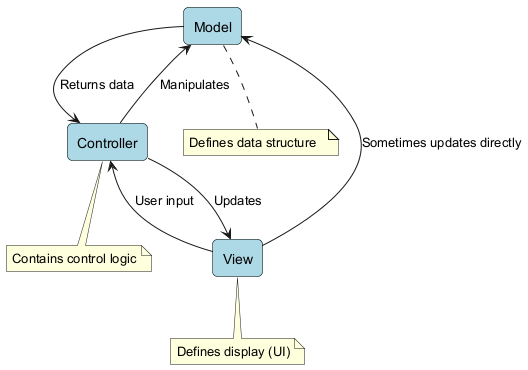
\includegraphics[width=0.45\textwidth]{png/MVC.png}} 
    \caption{Esquema del Model-Vista-Controlador.} 
    \label{fig:mvc} 
\end{figure}

El concepte de MVC va ser introduït per primera vegada per  \href{https://en.wikipedia.org/wiki/Trygve_Reenskaug}{Trygve Reenskaug}, qui el va proposar com una forma de desenvolupar el GUI d'aplicacions d'escriptori. Avui en dia, el patró MVC s'utilitza per a aplicacions web modernes perquè permet que l'aplicació sigui escalable, mantenible i fàcil d'expandir.

Les principals utilitats del patró MVC inclouen: 
\begin{itemize} 
    \item \textbf{Modularitat}: Facilita la separació de responsabilitats, permetent que cada component es desenvolupi i es mantingui de manera independent. Això respecta el principi de la responsabilitat única, on una part del codi no ha de saber què fa tota l'aplicació, només ha de tenir una responsabilitat específica.
    \item \textbf{Reutilització de codi}: Els components poden ser reutilitzats en diferents parts de l'aplicació o en altres projectes.
    \item \textbf{Facilitat de manteniment}: La separació de responsabilitats facilita la detecció i correcció d'errors, així com la implementació de noves funcionalitats.
    \item \textbf{Separació de preocupacions (SoC)}: El patró MVC ajuda a dividir el codi frontend i backend en components separats, fent que sigui molt més fàcil gestionar i fer canvis a qualsevol dels costats sense que interfereixin entre si.
\end{itemize}

El patró MVC és especialment útil quan diversos desenvolupadors necessiten actualitzar, modificar o depurar una aplicació completada simultàniament. Aquesta separació de preocupacions permet que els desenvolupadors treballin en diferents parts de l'aplicació sense afectar altres parts del codi. En el cas d'aquesta pràctica, podries canviar de vista o de solver i continuaria funcionant amb els nous components.

En resum, el patró MVC és una eina poderosa per a la construcció d'aplicacions escalables i mantenibles, permetent una clara separació de responsabilitats i facilitant la gestió del codi.

\subsection{Patró per Esdeveniments} 
El patró per esdeveniments és un mecanisme de comunicació entre components que permet gestionar esdeveniments i notificacions de manera eficient \cite{EventPattern}. En aquest patró, els components poden generar esdeveniments i subscriure's a esdeveniments generats per altres components.

\begin{itemize} 
    \item \textbf{Generació d'esdeveniments}: Els components poden generar esdeveniments quan es produeixen canvis en el seu estat o quan es completen determinades accions. En aquest projecte, per exemple, l'acció de prémer un botó per iniciar el càlcul de les distintes formes genera un esdeveniment que inicia l'execució dels càlculs. 
    \item \textbf{Subscripció a esdeveniments}: Els components poden subscriure's a esdeveniments generats per altres components per rebre notificacions i actuar en conseqüència.
 En l'aplicació, el Controlador s'encarrega de subscriure's als esdeveniments generats per la Vista (com un clic en un botó) per gestionar l'execució dels càlculs i actualitzar la Vista amb els resultats.
\item \textbf{Desacoblament}: El patró per esdeveniments permet desacoblar els components, ja que no necessiten conèixer els detalls dels altres components amb els quals interactuen. Això facilita l'escalabilitat i el manteniment de l'aplicació, ja que es poden afegir nous components o modificar els existents sense afectar la resta de l'aplicació. Per exemple, la Vista i el Model estan desacoblats, i el Controlador s'encarrega de gestionar la interacció entre ambdós a través dels esdeveniments.
\end{itemize}

\subsection{Càlcul del Cost Asimptòtic }
El càlcul del cost asimptòtic s'utilitza per analitzar l'eficiència dels algorismes en termes de temps d'execució i ús de memòria. Es basa en la notació Big-O, que descriu el comportament d'un algorisme a mesura que la mida de les dades d'entrada creix fins a l'infinit. Aquesta notació permet mesurar com s'incrementa el temps d'execució a mesura que augmenta la mida de l'entrada. Matemàticament, defineix el límit d'una funció quan els seus arguments tendeixen a l'infinit o a un valor determinat, representant el pitjor cas del temps d'execució en funció de la mida de les dades.\newline

La notació Big-O és important perquè permet als desenvolupadors i científics de dades avaluar i comparar l'eficiència de diferents algorismes. Això ajuda a triar l'algorisme més adequat per a una tasca específica, optimitzant el rendiment d'aplicacions i sistemes \cite{bigOAnalysis}.

\begin{figure}[htbp]
\centerline{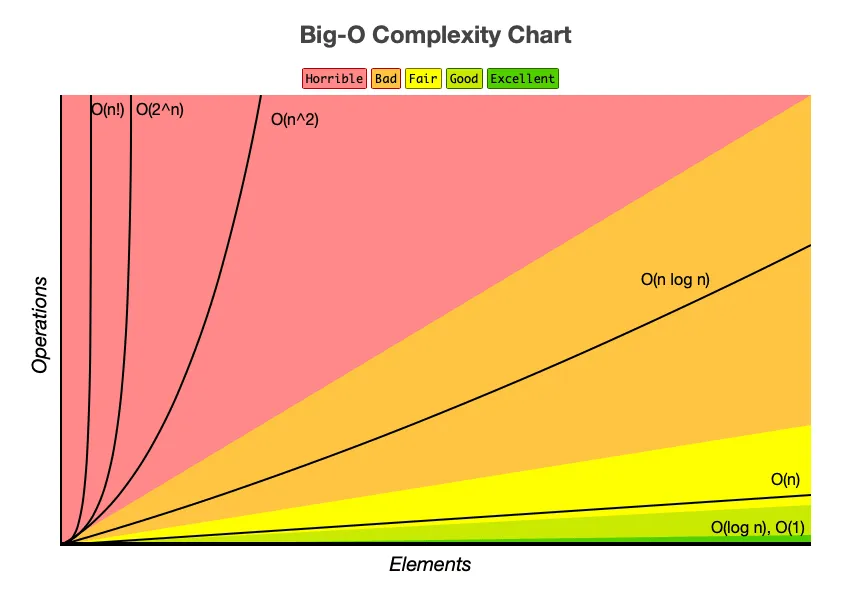
\includegraphics[width=0.45\textwidth]{png/bigO.png}}
\caption{Exemple de diferents complexitats de la notació Big-O.}
\label{fig:big_o}
\end{figure}

Per calcular la notació Big-O d'un algorisme, s'analitzen els bucles, bucles anidats, recursions i operacions dominants del codi, que són les que més afecten el temps d'execució. A més, un factor important que afecta el rendiment i l'eficiència del programa és el maquinari, el sistema operatiu i la CPU que s'utilitza. No obstant això, això no es té en compte quan s'analitza el rendiment d'un algorisme. En canvi, el que importa és la complexitat temporal i espacial en funció de la mida de l'entrada.

En resum, la notació Big-O és una eina essencial per avaluar l'eficiència dels algorismes i triar els més adequats per a cada situació, optimitzant així el rendiment de les aplicacions.

A la part d'analisi s'explicará amb detall el cost exponencial O(a\textsuperscript{n}), que és el propi dels algorismes desenvolupats en aquesta pràctica.
 
\subsection{Backtracking}
El backtracking és una tècnica algorísmica per resoldre problemes mitjançant l'exploració de diferents opcions de manera incremental. Si una elecció no condueix a una solució, es retrocedeix fins al punt de decisió anterior per provar una alternativa. Aquest enfocament és especialment útil en problemes que requereixen examinar múltiples possibilitats per trobar una solució vàlida o òptima. Quan s'arriba a un carreró sense sortida, l'algoritme torna enrere al punt de decisió anterior i explora un camí diferent fins que es troba una solució o s'han esgotat totes les possibilitats.

\begin{figure}[H]
\centering
\begin{lstlisting}[language=Java, basicstyle=\ttfamily\small]
boolean findSolutions(n, other params):
if (found a solution):
displaySolution();
return true;
for (val = first to last): 
    if (isValid(val, n)) :
        apply Value(val, n);
        if (findSolutions(n+1, other params))
            return true;
        removeValue(val, n);
    return false;
    
\end{lstlisting}

\caption{Esquema general d'una algorisme de backtracking}
\label{fig:f1}
\end{figure}

\subsection{Fractals  }
Un  fractal és una forma geomètrica que exhibeix autosimilitud, és a dir, la seva estructura es repeteix a diferents escales, de manera que una part ampliada conserva patrons similars a la forma global. A diferència de les figures geomètriques clàssiques, els fractals poden tenir una dimensió fractal no entera, situant-se entre les dimensions tradicionals, com entre una línia i una superfície. Es generen mitjançant processos iteratius o recursius, on una funció s'aplica repetidament, produint patrons d'alta complexitat. En programació, els fractals es construeixen amb funcions recursives, aplicació de fórmules matemàtiques iteratives (com en els conjunts de Mandelbrot i Julia \cite{sims}) o a través  sistemes de funcions iterades (IFS) \cite{ifs}) basats en transformacions geomètriques. Els fractals tenen múltiples aplicacions en informàtica, com en gràfics per ordinador per modelar paisatges i textures, en compressió d’imatges per reduir-ne la mida sense pèrdua de qualitat, en la simulació de fenòmens naturals com el creixement de plantes o la turbulència en fluids, i fins i tot en criptografia i anàlisi de dades, per a la generació de claus segures i la detecció de patrons complexos.
\section{Entorn de Programació}
Per al desenvolupament d'aquest projecte s'ha emprat un conjunt d'eines i tecnologies que han facilitat la implementació del patró MVC i l'anàlisi dels algorismes de suma i producte de matrius. A continuació, es descriuen les principals eines utilitzades:

\begin{itemize}
    \item \textbf{Llenguatge de programació: Java} \\
    Java és un llenguatge de programació orientat a objectes que ofereix una gran portabilitat i una àmplia gamma de llibreries i eines per al desenvolupament d'aplicacions. La seva sintaxi clara i la seva robustesa el fan ideal per a projectes que requereixen una alta mantenibilitat i escalabilitat. A més, Java és independent de la plataforma, la qual cosa permet executar l'aplicació en diferents sistemes operatius sense necessitat de modificar el codi.

    \item \textbf{Llibreries utilitzades: Swing} \\
    Swing és una llibreria de Java per a la creació d'interfícies gràfiques d'usuari (GUI). Proporciona un conjunt complet de components gràfics, com ara botons, camps de text, taules i panells, que permeten construir interfícies d'usuari riques i interactives. Swing és altament personalitzable i permet crear interfícies gràfiques que s'adapten a les necessitats específiques de l'aplicació.

    \item \textbf{IDE: IntelliJ IDEA} \\
    IntelliJ IDEA és un entorn de desenvolupament integrat (IDE) per a Java que ofereix una àmplia gamma de funcionalitats per a facilitar el desenvolupament d'aplicacions. Algunes de les seves característiques més destacades inclouen la completació de codi intel·ligent, la navegació ràpida pel codi, les eines de refactorització i la integració amb sistemes de control de versions. Aquestes funcionalitats ajuden a millorar la productivitat i a mantenir un codi net i organitzat.

    \item \textbf{Control de versions: GitHub} \\
    GitHub és una plataforma de desenvolupament col·laboratiu que utilitza el sistema de control de versions Git. Permet gestionar el codi font del projecte, fer seguiment dels canvis, col·laborar amb altres membres de l'equip i mantenir un historial complet de les modificacions realitzades. GitHub també ofereix eines per a la gestió de projectes, com ara issues i pull requests, que faciliten la coordinació i la revisió del codi.
\end{itemize}

L'ús d'aquestes eines i tecnologies ha permès desenvolupar una aplicació robusta i mantenible, seguint els principis del patró MVC i assegurant una bona gestió del codi i la col·laboració entre els membres de l'equip.

\section{Desenvolupament}
En aquesta secció es descriu el desenvolupament de la pràctica, que consisteix en la implementació d'una aplicació de dibuix de patrons geometrics basada en el patró Model Vista Controlador (MVC) i el patró per esdeveniments.

\subsection{Estructura}

\begin{itemize}
    \item \textbf{Model}: 
    Per a la gestió de les dades del programa, s'ha creat la classe \textbf{Dades}, que registra el tauler, element usat per guardar de forma intermedia, els resultats de dibuix dels algorismes implementats, un enum Tipus, que indica el tipus de peça que construeix un algorisme donat, la profunditat que tria l'usuari i una variable per guardar el valor de la constant multiplicativa.
    A part de la classe Dades, Model implementa també els algorismes per solucionar els següents problemes:
    Problema dels Tromins, problema dels triangles de Sierpinski, problema de l'estora de Sierpinski, i el dibuix recursiu d'arbres. A més, implementa una classe abstracta (\texttt{RecursiveSolver}) que implementen els \textbf{solvers} i que'ls permet utilitzar múltiples fils concurrents.
    \begin{itemize}
        \item\textbf{RecursiveSolver} Aquesta classe abstracta realitza l'encapsulament d'un \texttt{solver} per què pugui llançar fils de manera transparent.
    Per cada cridada recursiva es crea un fil, fet que permet augmentar la eficiencia del proces, però es necessària una gestio dels fils per a no saturar la CPU.
    És per a la gestió de fils s'utilitza un \texttt{ExecutorService} de tamany linealment variable amb el numero de nuclis de la CPU i una cua de \texttt{Runnable} de fils pendents d'executar.
    \end{itemize}
    
    

    \item \textbf{Vista}:
    Les classes \texttt{Finestra} i els distints \texttt{visualitzadors} s'encarreguen de la presentació de les dades a l'usuari. Utilitzen la llibreria Swing per crear la interfície gràfica i mostrar els resultats dels \texttt{solvers}.
    A més, els diferents \texttt{visualitzadors} implementen una classe abstracta que els permet executar-se en un propi fil amb un doble buffer.
\begin{itemize}
 \item\textbf{Finestra}
Aquesta classe representa la finestra principal de l'aplicació. Conté un \texttt{JComboBox} per seleccionar el tipus de visualització (tromino, triangles, quadrat i arbre), botons per executar, aturar, esborrar i activar/desactivar colors en la visualització, així com un camp de text per introduir valors numèrics i quatre botons per seleccionar els colors per a la visualització. Gestiona el canvi dinàmic entre diferents visualitzadors mitjançant la funció \texttt{replace(Comunicar nouDibuix)}.

\item \textbf{CanvasDobleBuffer}
Aquesta classe abstracta permet encapsular la lògica del doble buffer per als altres \texttt{visualitzadors}. La implementació utilitza un \texttt{BufferStrategy} i un fil que repinta el Canvas de forma periòdica, per exemple 60FPS. D'aquesta manera no es necessari que els \texttt{solvers} comuniquin un repintat a cada canvi, alliberant de carrega el procés de redibuixat.

\item\textbf{DibuixSierpinski}
Classe encarregada de dibuixar el Triangle de Sierpinski en un panell gràfic (\texttt{CanvasDobleBuffer}). Recorre una matriu de dades per determinar quins triangles ha de pintar i utilitza colors per diferenciar les profunditats de la figura. Inclou un "easter egg" per canviar el color a daurat en determinades condicions. \cite{easter_egg}
\item\textbf{DibuixTromino}
S'encarrega de representar la solució del problema dels Trominos. Dibuixa una quadrícula i pinta les peces dels trominos amb colors diferenciats quan l'opció de color està activada. També detecta clics de l'usuari per identificar caselles i enviar informació a la classe principal (\texttt{controlador.Main}).

\item \textbf{Altres:} Per pintar els resultats de l'estora i els arbres hi ha les dues classes encarregades, (\texttt{DibuixCarpet}) i (\texttt{DibuixImage}) respectivament.
\end{itemize}

\item\textbf{Controlador}
La classe \texttt{controlador.Main} actua com a controlador principal de l'aplicació, gestionant les interaccions de l'usuari i coordinant les operacions entre el model i la vista. També és responsable de la gestió de processos i de l'execució de les diferents funcionalitats.

\textbf{Elements principals}
\begin{itemize}
    \item \textbf{Inicialització}: 
    \begin{itemize}
        \item L'atribut \texttt{dades} representa el model de dades de l'aplicació.
        \item L'atribut \texttt{finestra} és la interfície gràfica, la qual permet a l'usuari interactuar amb el sistema.
        \item La llista \texttt{processos} conté els processos en execució.
        \item L'objecte \texttt{executor} és un \texttt{ExecutorService} amb un \textit{thread pool} de mida 16 per executar tasques en paral·lel.
    \end{itemize}
    
    \item \textbf{Creació i gestió dels components}:
    \begin{itemize}
        \item El mètode \texttt{init()} inicialitza les dades i els processos i crea la interfície gràfica en un fil separat mitjançant l'executor.
    \end{itemize}
    
    \item \textbf{Gestió de la matriu de dades}:
    \begin{itemize}
        \item El mètode \texttt{getMatriu()} retorna la matriu de dades.
        \item Quan es rep un missatge de tipus \texttt{"N"}, es crea una nova matriu de mida \(n \times n\) i es notifica la finestra perquè es redibuixi.
    \end{itemize}
    
    \item \textbf{Comunicació}:
    \begin{itemize}
        \item La classe \texttt{controlador.Main} implementa la interfície \texttt{Comunicar}, que defineix el mètode \texttt{comunicar}.
        \item Aquest mètode rep instruccions en forma de cadena de text i executa les accions corresponents mitjançant un sistema de control de missatges.
        \item Exemples de missatges:
            \begin{itemize}
                \item \texttt{"tempsReal"}, \texttt{"tempsEsperat"} $\rightarrow$ S'envien directament a la interfície gràfica.
                \item \texttt{"N:n"} $\rightarrow$ Es crea una nova matriu de mida \(n \times n\).
                \item \texttt{"inici"} $\rightarrow$ Es defineix el forat per a la resolució del problema dels trominos i s'inicia el càlcul.
            \end{itemize}
    \end{itemize}
    
    \item \textbf{Gestió de processos d'execució}:
    \begin{itemize}
        \item Quan es rep un missatge de tipus \texttt{"executar"}, la classe \texttt{controlador.Main} inicia el càlcul corresponent segons el tipus de visualització:
        \begin{itemize}
            \item \texttt{"tromino"}: Executa el solver dels Trominos.
            \item \texttt{"triangles"}: Executa el solver del Triangle de Sierpinski.
            \item \texttt{"quadrat"}: Executa el solver de l'estora de Sierpinski.
            \item \texttt{"arbre"}:  Executa el solver dels arbres
        \end{itemize}
        \item La creació i execució d'aquests processos es realitza mitjançant reflexió, instanciant dinàmicament les classes i executant-les en fils separats.
    \end{itemize}
    
    \item \textbf{Gestió de la finalització i neteja de processos}:
    \begin{itemize}
        \item Quan es rep el missatge \texttt{"aturar"}, s'atura l'execució de tots els processos en marxa.
        \item Amb el missatge \texttt{"borrar"}, s'atura tot, es netegen les dades i es redibuixa la interfície gràfica.
    \end{itemize}

\end{itemize}
També s'ha de comentar que la interfície \texttt{Comunicar} defineix el contracte bàsic per a la comunicació entre els diferents components de l'aplicació, i conté un únic mètode:

\begin{quote}
\texttt{void comunicar(String s);}
\end{quote}

Aquest mètode és utilitzat per transmetre missatges entre les diferents parts del sistema, especialment entre la vista (finestra gràfica), el controlador (\texttt{controlador.Main}) i el model (en aquest cas, la classe \texttt{Dades}). La interfície \texttt{Comunicar} és una eina fonamental per mantenir una separació clara entre la lògica de l'aplicació i la interfície d'usuari, permetent una comunicació eficient i flexible.

En resum, la classe \texttt{controlador.Main} és el nucli de l'aplicació, ja que actua com a intermediari entre la interfície gràfica i el model de dades. La seva estructura modular permet gestionar diferents tipus de visualitzacions i optimitzar el rendiment mitjançant execució concurrent.
\end{itemize}
\begin{figure}[htbp]
\centerline{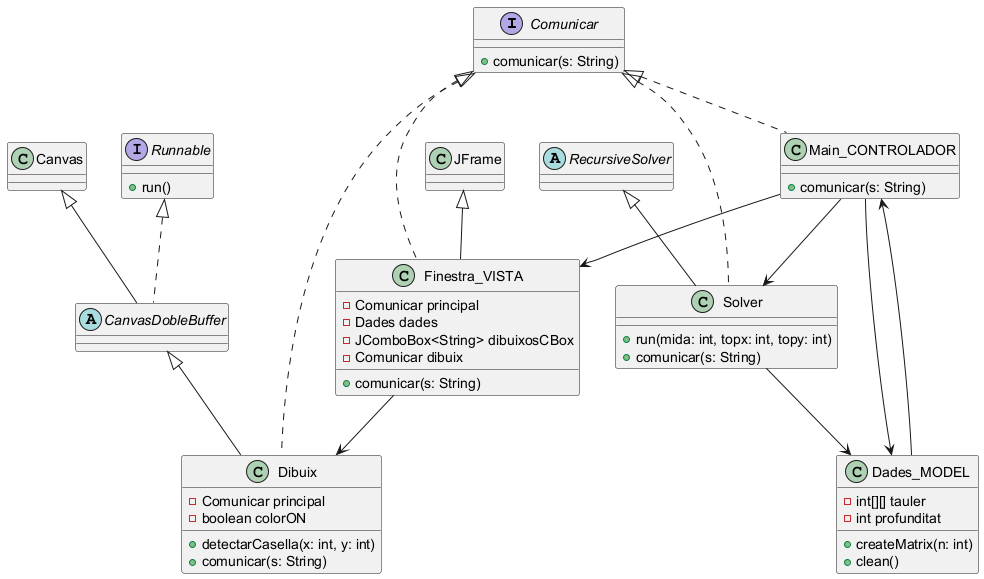
\includegraphics[width=0.45\textwidth]{docs/png/diagrma_clases.png}}
\caption{Diagrama molt senzill de classes.}
\label{fig:digC}
\end{figure}


\subsection{Implementació del Patró per Esdeveniments}
L'aplicació utilitza el patró per esdeveniments per gestionar la comunicació entre els components de manera eficient. Aquest patró permet que els components es comuniquin entre ells mitjançant l'enviament i la recepció de missatges, sense necessitat de conèixer els detalls interns dels altres components.

\subsubsection{Interfície \texttt{Comunicar}}
La interfície \texttt{Comunicar} defineix un mètode \texttt{comunicar} que permet enviar missatges entre els components. Aquesta interfície és implementada per diverses classes de l'aplicació, permetent una comunicació uniforme i consistent. La definició de la interfície és la següent:

\begin{lstlisting}[language=Java, basicstyle=\ttfamily\small]
public interface Comunicar {
    public void comunicar(String s);
}
\end{lstlisting}

\subsubsection{Classe \texttt{controlador.Main}}
La classe \texttt{controlador.Main} actua com a controlador central de l'aplicació i és responsable de gestionar la comunicació entre els components, com s'ha explicat anteriorment. Quan l'usuari interactua amb la interfície gràfica, la classe \texttt{controlador.Main} rep els missatges corresponents i els processa per iniciar, aturar o actualitzar les operacions de generació de figures. El mètode \texttt{comunicar} de la classe \texttt{controlador.Main} processa els missatges i crida als mètodes adequats per gestionar les operacions.

\subsubsection{Classes de \texttt{solvers}}
Tots els solvers implementen la interfície Comunicar per rebre missatges del controlador i aturar els fils d'execució quan sigui necessari. Quan es rep un missatge per aturar l’operació, el mètode comunicar d’aquestes classes estableix una variable booleana stop a true, la qual cosa fa que el mètode principal  s’aturi.
A més, estenen de la classe \textbf{RecursiveSolver} per poder executar concurrentment diversos fils.

\subsubsection{Classe \texttt{Finestra}}
La classe \texttt{Finestra} també implementa la interfície \texttt{Comunicar} per rebre missatges del controlador i actualitzar la interfície gràfica en conseqüència. Aquesta classe rep el missatge per comunicar i també l'envia a les classes de Dibuix per comunicar.
\subsubsection{Flux de Comunicació}
El flux de comunicació entre els components es pot resumir en els següents passos:

\begin{enumerate}
    \item L'usuari interactua amb la interfície gràfica mitjançant la classe \textsf{\texttt{Finestra}}, per exemple, seleccionant una opció del menú o introduint un valor per dibuixar una figura.
    \item La classe \texttt{Finestra} envia un missatge al controlador (\texttt{controlador.Main}) mitjançant el mètode \texttt{comunicar}.
    \item El controlador (\texttt{controlador.Main}) processa el missatge i, si és necessari, executa un procés concret (per exemple, \texttt{TrominoSolver}, \texttt{SierpinskiSolver}, \texttt{RecursiveTree} o \texttt{CarpetSierpinski}) en un fil separat utilitzant un \texttt{ExecutorService}.
    \item Els solucionadors (\texttt{TrominoSolver}, \texttt{SierpinskiSolver}, etc.) realitzen els càlculs corresponents en paral·lel i, durant l'execució, envien missatges al controlador per actualitzar l'estat del procés.
    \item El controlador informa la interfície gràfica (\texttt{Finestra}) sobre l'estat de l'execució mitjançant missatges com \texttt{tempsReal} o \texttt{tempsEsperat}.
    \item Quan un procés finalitza o es rep un missatge per aturar-lo, aquest comunica al controlador la seva terminació (\texttt{aturar}), i aquest ho notifica a la interfície perquè actualitzi els resultats.
    \item La interfície gràfica (\texttt{Finestra}) utilitza la classe \texttt{DibuixTromino} , per exemple, per actualitzar la visualització de la figura calculada.
\end{enumerate}

Aquesta arquitectura basada en missatges garanteix la separació de responsabilitats entre la interfície, el controlador i els processos de càlcul, permetent una execució eficient i flexible de les operacions.

\subsection{Solvers}
En aquesta secció, abordarem de manera detallada els algorismes \textit{solvers}. En general, tenen la següent estructura:

\begin{enumerate}
    \item Implementació d'un mètode recursiu que resol el problema donat.
    \item Implementació del mètode per al cas base, que inclou l'emmagatzematge de les dades als taulers.
    \item Implementació del mètode \texttt{run()}, ja que els \textit{solvers} es basen en fils d'execució.
    \item Implementació del mètode \texttt{stop()}, per aturar l'execució dels fils.
    \item Finalment, implementació del mètode \texttt{communicar()}, per la comunicació entre fils o components.
\end{enumerate}

\subsubsection{TrominoSolver}
Aquesta classe soluciona el següent problema; donat un tauler de mida exponencial \(2^n\), i amb un forat en qualsevol posició \((x,y)\) del tauler, omple el tauler amb tromins de forma recursiva.
Aquest algoritme segueix l'estratègia de divideix i venceràs, fragmentant el tauler en quadrants més petits fins a aconseguir una mida mínima de \(2x2\). Per a cada subdivisió, localitza la posició del forat existent i col·loca un tromino central per a garantir una cobertura completa del tauler. A mesura que avança la recursió, l'algoritme executa múltiples fils per resoldre simultàniament les diferents regions del tauler, millorant així el rendiment en entorns de processament paral·lel. Al final de l'execució, es mesura el temps emprat i es calcula una constant multiplicativa basada en la profunditat del tauler, la qual permet estimar el temps d'execució per a futures execucions.

\begin{figure}[htbp]
\centerline{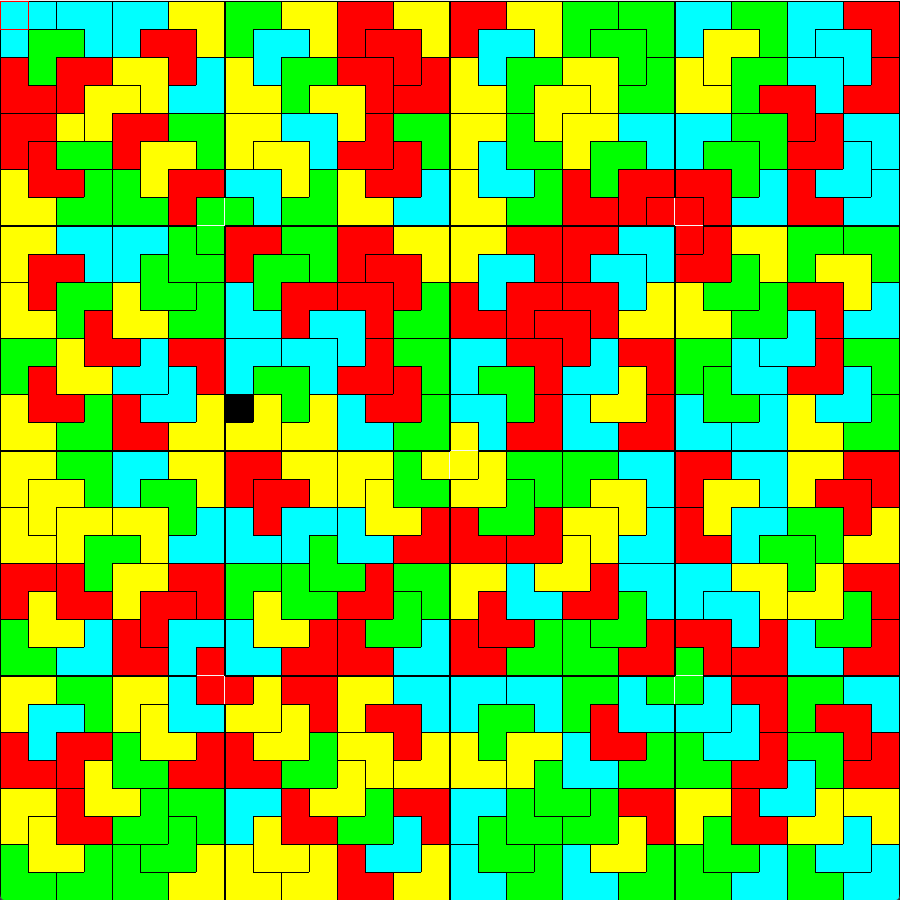
\includegraphics[width=0.4\textwidth]{docs/png/FiguraTromino5.png}}
\caption{Exemple d'un tromino de profunditat 5.}
\label{fig:int2}
\end{figure}

\subsubsection{SierpinskiTriangleSolver}
La fractal dels triangles de Sierpinski tracta de dividir un triangle en tres triangles més petits de manera recursiva, eliminant el triangle central en cada iteració. Aquest procés continua fins que s'arriba a un nivell de profunditat determinat.

La classe SierpinskiTriangleSolver resol aquest problema aplicant recursivitat per generar la figura. Comença amb un triangle gran i divideix recursivament l'espai en tres sub-triangles fins que la mida mínima s'assoleix. La classe utilitza un tauler bidimensional int[][] tauler per representar la figura i marca les posicions corresponents amb data.setValor(x, y, 1). L'execució es fa de manera asíncrona mitjançant fils (runThread), permetent una representació dinàmica de la construcció del fractal. A més, mesura el temps d'execució i estima el temps esperat basant-se en la profunditat de recursió, comunicant la informació a través de p.comunicar, sent p la instància del Programa principal controlador.Main.

\begin{figure}[htbp]
\centerline{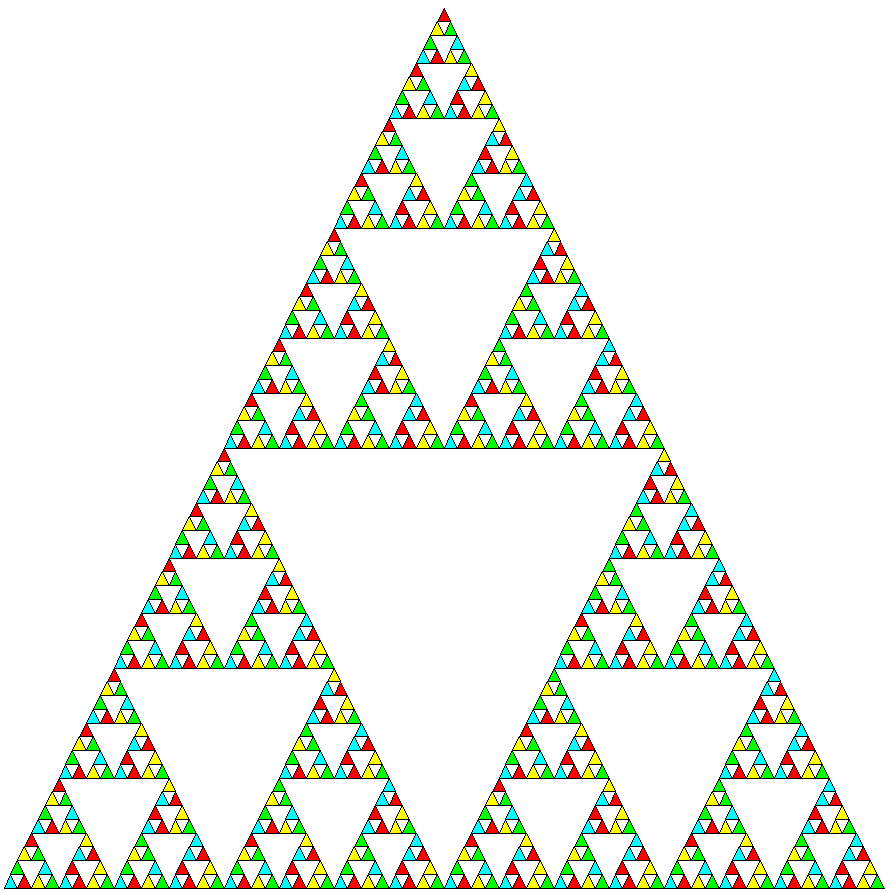
\includegraphics[width=0.4\textwidth]{docs/png/FiguraTriangle7.png}}
\caption{Exemple d'un triangle de profunditat 7.}
\label{fig:int2}
\end{figure}


\subsubsection{SierpinskiCarpetSolver}
L'estora de Sierpinski és una fractal que segueix un patró consistent en dividir un quadrat en nou quadrats de mida igual, realitzant tres divisions horitzontals i tres verticals. Tots els quadrats es pinten, excepte el central.

L'algorisme recursiu de la classe implementa exactament aquest procés. Pel que fa al tauler, es va omplint amb valors enters incrementals que representen els quadrats, establint l'ordre en què han de ser pintats.

\begin{figure}[htbp]
\centerline{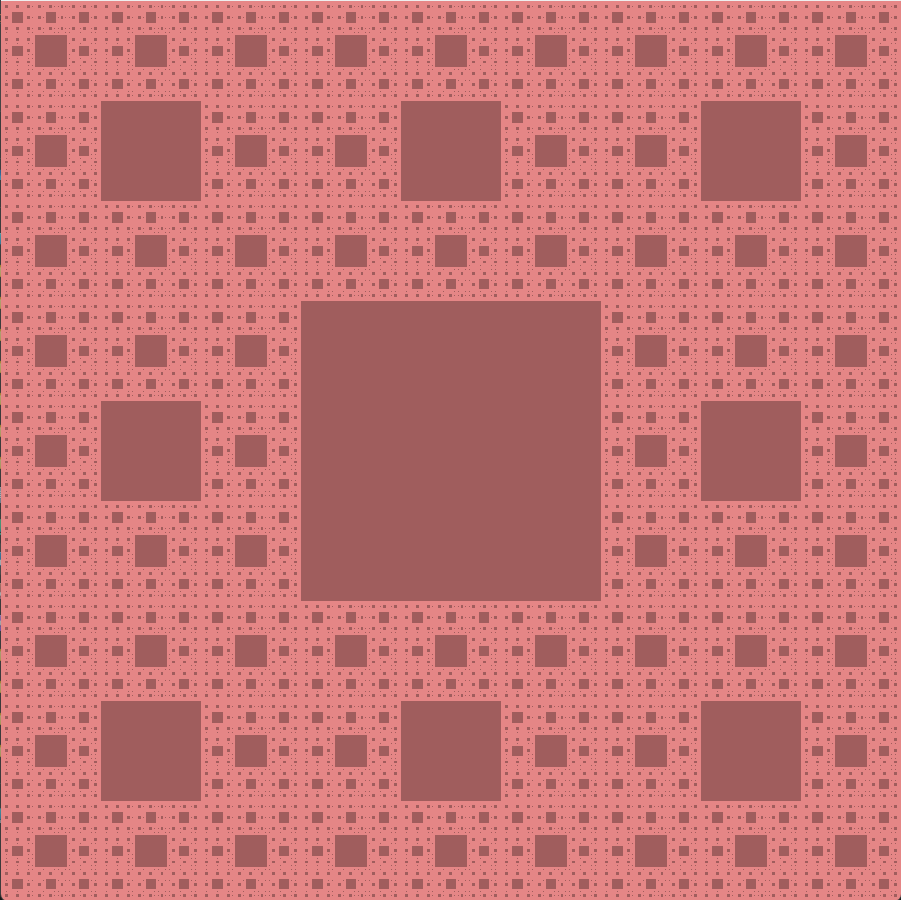
\includegraphics[width=0.4\textwidth]{docs/png/FiguraEstora6.png}}
\caption{Exemple d'un estora de profunditat 6.}
\label{fig:int2}
\end{figure}

\subsubsection{TreeSolver}
Es tracta de dibuixar un arbre de forma recursiva. L'element base de l'arbre és la branca, i a mesura que s'incrementa la profunditat, les arrels es van afegint de manera exponencial.

La implementació de l'algorisme utilitza dues propietats geomètriques trivials per calcular les posicions de les branques, tenint en compte el seu angle d'inclinació i la seva longitud.

\begin{lstlisting}[language=Java, basicstyle=\ttfamily\small]
 int x2 = x1 + (int) (Math.cos(Math.toRadians(angle)) * treeLogSize );
 int y2 = y1 + (int) (Math.sin(Math.toRadians(angle)) * treeLogSize);
\end{lstlisting}

\begin{figure}[htbp]
\centerline{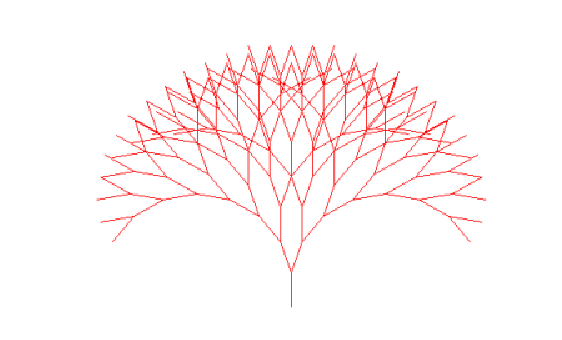
\includegraphics[width=0.4\textwidth]{docs/png/tree.png}}
\caption{Exemple d'un arbre recursiu de profunditat 8.}
\label{fig:int2}
\end{figure}

Ara bé, aquest model no representa la figura de l'arbre en forma de matriu, sinó com una imatge de tipus \texttt{BufferedImage} de mida personalitzada.


\subsection{Interfície Gràfica}
L'aplicació utilitza la llibreria Swing per crear una interfície gràfica que permet a l'usuari seleccionar i visualitzar diferents figures geomètriques recursives. L'usuari pot triar entre trominos, triangles de Sierpinski, quadrats i arbres, així com modificar l'aparença dels dibuixos canviant els colors o actualitzant la representació.
\subsubsection{Classes de Dibuix}
Les classes de \texttt{Dibuix} s'encarregen de representar gràficament la solució del problema. Aquestes classe implementen la interfície \texttt{Comunicar} per comunicar-se amb la classe principal i actualitzar la visualització i estenen \texttt{CanvasDobleBuffer} per al doble buffer.\newline

Per exemple, la classe \texttt{DibuixTromino} s'encarrega de dibuixar la matriu solució del solver. Els elements principals d'aquesta classe són:
\begin{itemize}
\item \textbf{Pintura i dibuix}: Utilitza el mètode \texttt{pintar()} per dibuixar la matriu de trominos sobre el panell gràfic.
\item \textbf{Detecció d'interacció}: Implementa un \texttt{MouseListener} per detectar clics a la graella i comunicar la posició seleccionada a la classe principal.
\item \textbf{Colorejat dinàmic}: Assigna colors diferents als trominos depenent de la selecció previa.
\item \textbf{Dibuix de vores}: Dibuixa només les vores exteriors dels trominos per millorar la claredat visual.
\end{itemize}

\subsubsection{Classe Finestra}
La classe \texttt{Finestra} és responsable de crear la interfície gràfica principal de l'aplicació. Aquesta classe utilitza diversos components de Swing per permetre a l'usuari seleccionar diferents figures i interactuar amb la visualització.\newline

Els elements principals de la interfície inclouen:
\begin{itemize}
\item \textbf{ComboBox de selecció}: Un \texttt{JComboBox} que permet seleccionar entre trominos, triangles de Sierpinski, quadrats i arbre.
\item \textbf{Botons d'acció}: Inclou botons per pintar, aturar l'execució, esborrar la visualització i canviar els colors dels dibuixos.
\item \textbf{Camp de text per paràmetres}: Un \texttt{JTextField} on l'usuari pot introduir valors per definir la mida de la figura generada.
\item \textbf{Gestió dinàmica de components}: Quan es selecciona una nova figura, es reemplaça el panell de dibuix anterior per un de nou sense reiniciar tota la interfície.
\end{itemize}

\subsubsection{Comunicació entre classes}
Les classes \texttt{DibuixTromino} i \texttt{Finestra} es comuniquen mitjançant la interfície \texttt{Comunicar}, que permet enviar missatges per actualitzar l'estat de la interfície i la representació gràfica.

\subsection{Gestió de Fils d'Execució}
La classe \texttt{controlador.Main} utilitza un \texttt{ExecutorService} per gestionar els fils d'execució dels distints solvers. Això permet executar les operacions de manera concurrent i millorar l'eficiència de l'aplicació. Els fils es poden iniciar i aturar mitjançant missatges enviats a través de la interfície \texttt{Comunicar}.
\subsubsection{ExecutorService}
L'\texttt{ExecutorService} és una interfície que proporciona mecanismes per gestionar un conjunt de fils d'execució. En aquest projecte, s'utilitza per executar els distints solvers en fils separats\cite{oracleExecutorService}. La classe \texttt{controlador.Main} crea un \texttt{ExecutorService} amb un grup de fils fixos mitjançant el mètode \texttt{Executors.newFixedThreadPool(16)}:
\begin{lstlisting}[language=Java, basicstyle=\ttfamily\small]
executor = Executors.newFixedThreadPool(16);
\end{lstlisting}
Això permet tenir fins a 16 fils d'execució simultanis, assegurant que les operacions de càlcul i resolució de problemes es puguin executar de manera concurrent.

\begin{figure}[htbp]
\centerline{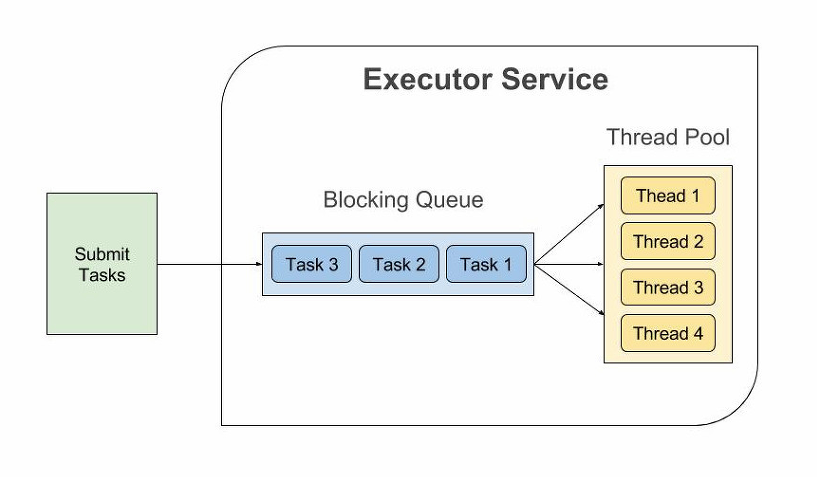
\includegraphics[width=0.45\textwidth]{png/executorService.png}}
\caption{Esquema de funcionament de l'Executor Service a Java.}
\label{fig:exeServ}
\end{figure}

\subsubsection{Inici i Aturada de Fils}
Quan l'usuari interactua amb la interfície gràfica per iniciar una operació, la classe \texttt{controlador.Main} rep un missatge mitjançant el mètode \texttt{comunicar}. Aquest mètode processa el missatge i, si és necessari, crea instàncies de les classes \texttt{TrominoSolver}, \texttt{SierpinskiSolver}, \texttt{RecursiveTree} o \texttt{CarpetaSierpinski} per executar les operacions en fils separats. Per exemple, quan es rep un missatge per iniciar l'execució del Tromino Solver, es crea i s'executa una instància de la classe corresponent en un fil separat:

\begin{lstlisting}[language=Java, basicstyle=\ttfamily\small]
TrominoSolver trominoTask = new TrominoSolver(this, dades);
processos.add(trominoTask);
executor.execute(trominoTask);
\end{lstlisting}

D'aquesta manera, les operacions es realitzen de forma concurrent, aprofitant els recursos disponibles per millorar el rendiment de l'aplicació.

\subsubsection{Casos de Concurrència}
L'aplicació pot gestionar diferents casos de concurrència, depenent de les operacions que l'usuari decideixi executar:

\begin{itemize}
   
    \item \textbf{Execució de Solvers Específics}: Quan l'usuari decideix executar un solver, com per exemple el Tromino Solver, es crea i executa una instància d'aquest solver en un fil separat, aturant l'anterior:


    \begin{lstlisting}[language=Java, basicstyle=\ttfamily\small]
    Comunicar proces = (Comunicar) classe
        .getConstructor(controlador.Main.class, Dades.class)
        .newInstance(this, dades);
    processos.add(proces);
    executor.execute((Runnable) proces);
    \end{lstlisting}
\end{itemize}

\subsubsection{Aturada de Fils}
Quan es rep un missatge per aturar una operació, el mètode \texttt{comunicar} de la classe \texttt{controlador.Main} envia un missatge a les instàncies dels solvers per aturar els fils d'execució. Això es fa establint la variable booleana \texttt{stop} a \texttt{true}, la qual cosa fa que el bucle principal de cada solver s'aturi de forma controlada. Per exemple:

\begin{lstlisting}[language=Java, basicstyle=\ttfamily\small]
for (Comunicar enmarxa : processos) {
    enmarxa.comunicar("aturar");
}
\end{lstlisting}

Això assegura que les operacions es puguin aturar de manera controlada i que els recursos es puguin alliberar correctament.
\subsubsection{Implementació de la Classe \texttt{controlador.Main}}
La classe \texttt{controlador.Main} és la responsable de gestionar els processos i filtrar els missatges. A continuació es mostra una part de la classe \texttt{controlador.Main}, que inclou la gestió d'operacions en fils d'execució:

\begin{lstlisting}[language=Java, basicstyle=\ttfamily\small]
public class controlador.Main implements Comunicar {

    private Comunicar finestra;
    private Dades dades;
    private ArrayList<Comunicar> processos = null;
    private final ExecutorService executor = Executors.newFixedThreadPool(16);

    public void comunicar(String s) {
        String[] params = s.split(":");
        switch (params[0]) {
            case "executar":
                switch (params[1]) {
                    case "tromino":
                        executar(TrominoSolver.class, (int) Math.pow(2, Integer.parseInt(params[2])));
                        break;
                    case "triangles":
                        executar(SierpinskiSolver.class, (int) Math.pow(2, Integer.parseInt(params[2]) - 1));
                        break;
                      [...]
                    // altres operacions
                }
                break;
            case "aturar":
                for (Comunicar proces : processos) {
                    proces.comunicar("aturar");
                }
                break;
            [...]
            // altres casos
        }
    }

    private void executar(Class<? extends Comunicar> clase, int profunditat) throws NoSuchMethodException, InvocationTargetException, InstantiationException, IllegalAccessException {
        for (Comunicar enmarxa : processos) {
            enmarxa.comunicar("borrar");
        }
        processos.clear();
        dades.setProfunditat(profunditat);
        Comunicar proces = (Comunicar) clase.getConstructor(controlador.Main.class, Dades.class).newInstance(this, dades);
        processos.add(proces);
        executor.execute((Runnable) proces);
    }
}
\end{lstlisting}

\subsubsection{Conclusió}
L'ús de l'\texttt{ExecutorService} en la classe \texttt{controlador.Main} i \texttt{RecursiveSolver} per gestionar els fils d'execució és fonamental per a la implementació concurrent de les operacions. Aquesta gestió permet a l'aplicació realitzar càlculs intensius de manera eficient, millorant el rendiment i mantenint l'aplicació responsiva. Gràcies a la separació de les operacions en fils independents, es garanteix una bona escalabilitat i flexibilitat del sistema.

També gràcies al \textbf{MVC} ha estat possible implementar de forma independent els \textbf{solvers} com els \textbf{visualitzadors}, permetent una millora continua d'un sense perill de rompre l'altre.

\section{Resultats i Anàlisi}
En aquesta secció, analitzarem el cost asimptòtic dels algorismes implementats i compararem el temps real d'execució amb el temps estimat a partir de la constant multiplicativa.  

Per a aquest anàlisi, executarem cada algorisme amb diferents valors de profunditat \( n \) i recopilarem els resultats.  

Les gràfiques següents il·lustren els resultats obtinguts.
\begin{figure}[h]
\centerline{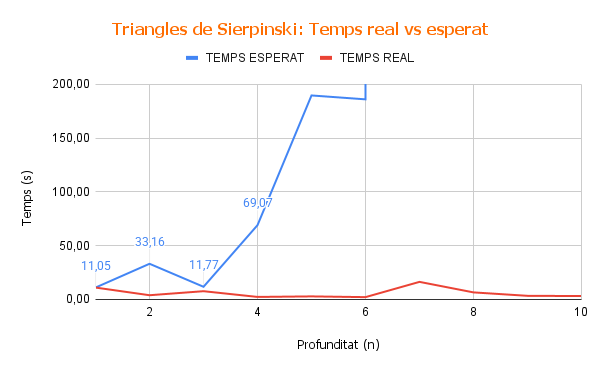
\includegraphics[width=0.4\textwidth]{docs/png/Triangles de Sierpinski_ Temps real vs esperat.png}}
\caption{Triangles de Siperpinski: Temps real vs esperat}
\label{fig:int2}
\end{figure}
\begin{figure}[H]
\centerline{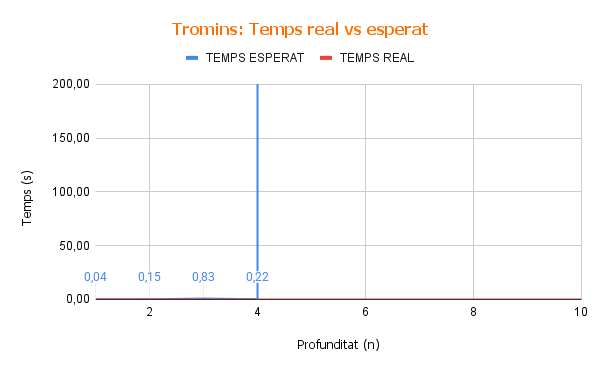
\includegraphics[width=0.4\textwidth]{docs/png/Tromins_ Temps real vs esperat.png}}
\caption{Tromins: Temps real vs esperat}
\label{fig:int2}
\end{figure}
\begin{figure}[H]
\centerline{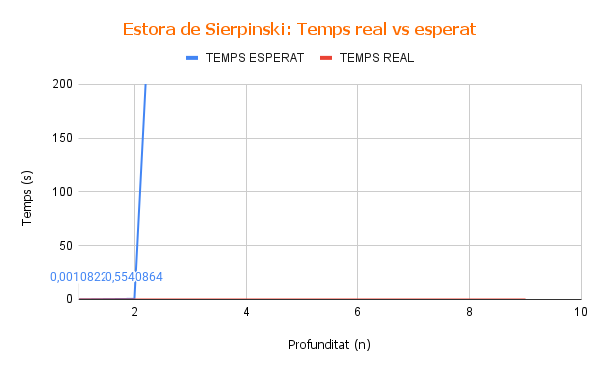
\includegraphics[width=0.4\textwidth]{docs/png/Estora de Sierpinski_ Temps real vs esperat.png}}
\caption{Estora de Sierpinski: Temps real vs esperat}
\label{fig:int2}
\end{figure}
\begin{figure}[H]
\centerline{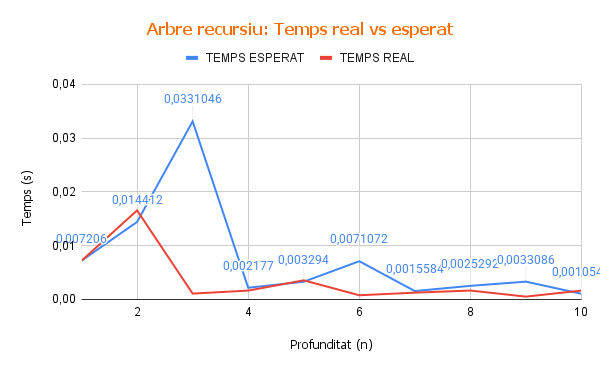
\includegraphics[width=0.4\textwidth]{docs/png/Arbre recursiu_ Temps real vs esperat.png}}
\caption{Arbre recursiu: Temps real vs esperat}
\label{fig:int2}
\end{figure}

Començant pels triangles de Sierpinski, el cost computacional del seu algorisme és de \( O(3^{n/2}) \), fent tres crides recursives, i en cada cridada el conjunt \( n \) es redueix a la meitat. Això implica que, a mesura que augmenta \( n \), el nombre de subdivisions creix exponencialment, fent que el cost computacional es dispari i limitant la profunditat màxima viable per a la seva representació gràfica.\newline

La constant multiplicativa usada per als càlculs estimats s'actualitza en cada execució fins que arriba a estabilitzar-se. Tot i això, s'observa que a partir de \( n = 6 \), el temps esperat es torna tan gran que ja no es pot apreciar en la gràfica, i per als  darrers valors de profunditat, \( n = 9 \) i \( n = 10 \), el temps calculat tendeix a l'infinit, fent impossible la seva generació en temps raonable.

No obstant això, a la pràctica, el temps d'execució real de l'algorisme és gairebé lineal, amb una complexitat efectiva de \( O(n) \). Ja que el procés d'omplir la matriu representativa és lineal, tenguint en compte que cada punt es marca només una vegada sense recomputacions innecessàries.\newline

Per altra banda, el dibuix dels trominos i de l'estora de Sierpinski esdevé intractable fins i tot per a valors baixos de profunditat, a causa del seu cost computacional elevat: \( O(4^{n/2}) \) i \( O(8^{n/3}) \), respectivament. L'algorimse de solucionar els tromins, per una banda, redueix el conjunt n a la meitat en cada cridada recursiva, i llança quatre crides a ell mateix per omlipr els  quatre quadrants nous. Per altra banda, l'algorisme de l'estora de Sierpinski, fa tres divisions verticals i altres 3 horizontals, de manera que obtenguim 9 quadrants de la mateixa mida, i el procés es repeteix fins que la profunditat sigui 1.\newline 

Finalment, l'\textbf{arbre recursiu} té el menor cost computacional, ja que es basa en una representació diferent-dibuixa directament les lines sobre un bufferedImage-, amb una complexitat de \( O(2^n) \). Això explica per què els temps esperats són molt inferiors als altres casos, fent que aquest algorisme sigui més escalable per a valors més grans de \( n \).\newline

Per poder ordenar els algorismes, segons el seu cost computacional, calcularem per deu conjunts diferents els valors del costs computacionals respectius dels algorismes.

\begin{table}[h]
    \centering
    \begin{tabular}{|c|c|c|c|c|}
        \hline
        \textbf{N} & \textbf{Arbre} & \textbf{Estora} & \textbf{Tromino} & \textbf{Triangle} \\
        \hline
        1  & 2,00    & 2,00      &  2,00  & 1,73  \\
        2  & 4,00    & 4,00      &  4,00  & 3,00  \\
        3  & 8,00    & 8,00     &  8,00  & 5,20  \\
        4  & 16,00   & 16,00     & 16,00  & 9,00  \\
        5  & 32,00   & 32,02    & 32,00 & 15,59 \\
        6  & 64,00   & 64,00    & 64,00 & 27,00 \\
        7  & 128,00  & 128,00  & 128,00 & 46,77 \\
        8  & 256,00  & 256,00  & 256,00 & 81,00 \\
        9  & 512,00  & 512,00 & 512,00 & 140,30 \\
        10 & 1.024,00 & 1.024,00 & 1024,00 & 243,00 \\
        \hline
    \end{tabular}
    \vspace{5mm}
    \caption{Comparació dels temps exponencials dels quatre algoritmes}
    \label{tab:complexitat}
\end{table}

Segons la taula obtinguda, s'observa que l'algorisme per resoldre els arbres recursius, l'estora de Sierpinski i els tromins tenen el mateix cost. En canvi, el solucionador dels triangles de Sierpinski varia una mica i resulta ser més eficient.

Per tant, l'ordenació dels algorismes queda de la següent manera:

\[
\boxed{O(3^{n/2}) < O(4^{n/2}) = O(2^n) = O(8^{n/3})}
\]



Així té molt de sentit, perquè si desenvolupem les expressions obtenim el següent:  
\[\boxed{
8^{(n/3)} = (2^3)^{(n/3)} = 2^n}
\]  
\[\boxed{
4^{(n/2)} = (2^2)^{(n/2)} = 2^n
}\]


Per últim, donada la rapidesa amb què creix la complexitat d'aquests algorismes, es fa evident que només es poden visualitzar per a valors petits de \( n \) abans que el temps d'execució sigui prohibitiu.
Tampoc té molt de sentit executar aquests algorismes amb \(n \) grans ja que no es podria visualitzar el resultat per falta de resolució.

\section{Conclusions}  
Aquesta pràctica s’ha dut a terme en aproximadament una setmana. Al començament, es van repartir els rols, però no hi havia una indicació clara sobre com implementar els elements perquè es poguessin comunicar entre ells. A més, la manca de comunicació entre alguns membres de l’equip va provocar que es dupliqués feina en els models, fent que dues persones desenvolupessin diferents implementacions dels models de Tromino i dels triangles de Sierpinski.

Per resoldre aquesta situació, es va convocar una segona reunió on, aquesta vegada, es va definir de manera més clara com s’havien de plantejar els models solvers i com es comunicarien amb el controlador i la vista.

Una de les dificultats principals ha estat la representació dels fractals en una estructura de matriu. Això ha requerit un enfocament específic per garantir que la divisió i la propagació de les subestructures es fes correctament. En el cas del model de l'arbre recursiu, s'ha optat per un altre plantejament: en lloc de treballar directament sobre una matriu, la figura es dibuixa sobre un BufferedImage, i posteriorment s'escala aquesta imatge per adaptar-la a la mida desitjada, com s'ha explicat previament a la memòria.

A més, una de les complexitats més destacades ha estat la implementació del controlador i la gestió de la comunicació entre totes les classes del programa. Ha estat necessari definir un mecanisme eficient perquè els diferents models enviessin la informació correcta a la vista sense generar inconsistències. En particular, la representació de les solucions tant dels triangles de Sierpinski com dels trominos dins una matriu ha suposat un desafiament addicional, ja que s’ha hagut de garantir que cada element quedés correctament posicionat i identificat per ser posteriorment representat gràficament.

Altres característiques que varen presentar un desafiu va ser l'execució concurrent de les cridades recursives. És cert que utilitzar un \texttt{ExecutorService} va simplificar molt el problema, però va ser necessària la implementació d'una cua per no sobrecarregar el sistema, tenint molta cura de no provocar cap bloqueig.

Respecte a l'organització del treball, l'equip va repartir les tasques de manera estructura, com indica la següent figura il·lustrativa.

\begin{figure}[htbp]
\centerline{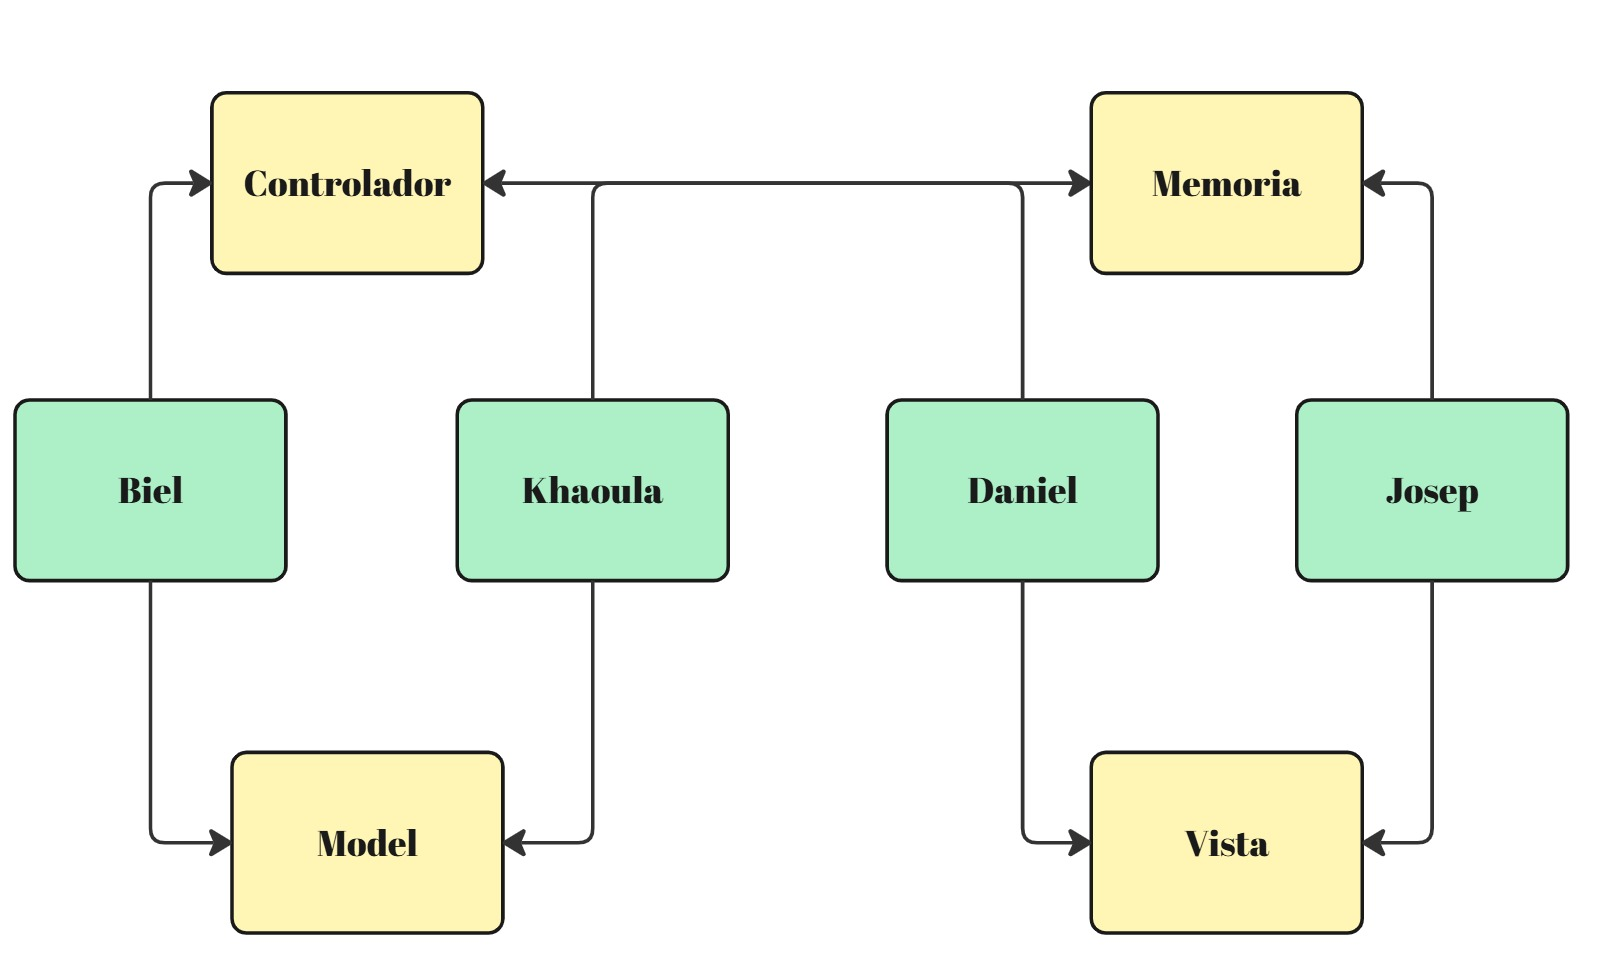
\includegraphics[width=0.4\textwidth]{docs/png/Repartiment.jpg}}
\caption{Repartiment de feina entre l'equip}
\label{fig:int2}
\end{figure}

Cada parella ha treballat en una part específica de la pràctica. Na Khaoula i en Biel s'han encarregat del Model, en Daniel i en Josep de la Vista, en Daniel i en Biel del Controlador, i na Khaoula i en Josep de la Memòria. A la vida real, així va ser la distribució, tot i que també és cert que els membres de l'equip han realitzat petites modificacions en les parts de la feina dels seus companys.

Pel que fa al feedback sobre aquesta pràctica, la majoria de l’equip ha trobat il·lusionant poder visualitzar el resultat final dels models implementats, fet que també ha motivat a seguir-ne desenvolupant més. A més, per a molts membres, aquesta pràctica ha estat la seva primera experiència programant el dibuix de fractals, cosa que ha fet que el treball tingui una gran utilitat tant a nivell d’aprenentatge com de motivació.

\begin{thebibliography}{9}

\bibitem{oracle_bufferstrategy}
Oracle, \textit{Full-Screen Exclusive Mode and BufferStrategy}, \url{https://docs.oracle.com/javase/tutorial/extra/fullscreen/bufferstrategy.html}, Accedido: 2025-03-25.

\bibitem{wikiFractal}
Wikipedia. (s.f.). \textit{Fractal}. Recuperat de: \url{https://en.wikipedia.org/wiki/Fractal}


\bibitem{bigOAnalysis}
GeeksforGeeks. (2021). \textit{Analysis of Algorithms | Big-O Analysis}. Recuperat de: \url{https://www.geeksforgeeks.org/analysis-algorithms-big-o-analysis/}

\bibitem{geeksFractals}
GeeksforGeeks. (s.f.). \textit{Fractals in C++}. Recuperat de: \url{https://www.geeksforgeeks.org/fractals-in-cc/}

\bibitem{sims} Sims, K. (1999). \textit{Julia Sets}. Recuperat de \url{https://www.karlsims.com/julia.html}

\bibitem{ifs} ScienceDirect. (s.f.). \textit{Iterated Function System}. Recuperat de \url{https://www.sciencedirect.com/topics/mathematics/iterated-function-system#:~:text=Iterated%20function%20systems%20(IFS)%20are,substantial%20industry%20of%20image%20compression.}

\bibitem{easter_egg} Wikipedia (s.f). \textit{El easter egg fa referencia a la Triforça de la reconeguda saga de videojocs de Nintendo "The Legend of Zelda"}. Recuperat de \url{https://en.wikipedia.org/wiki/Triforce}

\bibitem{MVC_Theory}
Trygve Reenskaug, "The Model-View-Controller (MVC) Pattern," \textit{Software Engineering Notes}, vol. 10, no. 6, pp. 1-3, Dec. 1985. [En línia]. Disponible: \url{https://en.wikipedia.org/wiki/Trygve_Reenskaug}.

\bibitem{mvcPattern}
GeeksforGeeks. (2021). \textit{MVC Design Pattern}. Recuperat de: \url{https://www.geeksforgeeks.org/mvc-design-pattern/}

\bibitem{mvcBenefits}
GeeksforGeeks. (2021). \textit{Benefit of Using MVC}. Recuperat de: \url{https://www.geeksforgeeks.org/benefit-of-using-mvc/}

\bibitem{Backtracking}
D. E. Knuth, \textit{The Art of Computer Programming, Volume 1: Fundamental Algorithms}, 3rd ed., Reading, MA: Addison-Wesley, 1997.

\bibitem{EventPattern} 
Eric Gamma, Richard Helm, Ralph Johnson, and John Vlissides. \emph{Design Patterns: Elements of Reusable Object-Oriented Software}. Addison-Wesley, 1994.

\bibitem{SwingLibrary}
Oracle, "Swing: A GUI Widget Toolkit," \textit{Oracle Documentation}, Oracle Corporation, 2009. [En línia]. Disponible: \url{https://docs.oracle.com/javase/8/docs/api/javax/swing/package-summary.html}.

\bibitem{oracleExecutorService}
Oracle. (2014). \textit{ExecutorService Interface (Java Platform SE 8)}. Recuperat de: \url{https://docs.oracle.com/javase/8/docs/api/java/util/concurrent/ExecutorService.html}

\end{thebibliography}

\end{document}


